\documentclass[czech]{beamer}
% Class options include: notes, notesonly, handout, trans,
%                        hidesubsections, shadesubsections,
%                        inrow, blue, red, grey, brown
%\setbeamertemplate{footline}[page number]
\mode<presentation> {
  
  \usetheme{Warsaw}
 %\setbeamertemplate{footline}{\hfill\insertframenumber/\inserttotalframenumber}
  \setbeamercovered{transparent}
% 	\setbeamertemplate{footline}
%	{
%		\insertpagenumber
%	}
 
  %\setbeamertemplate{footline}{\hfill\insertframenumber/\inserttotalframenumber}
  
  %\setbeamertemplate{footline}[page number] 
}

% Theme for beamer presentation.
\usepackage[T1]{fontenc}
\usepackage[utf8]{inputenc} 
\usepackage[czech]{babel}
\usepackage{multirow}
\usepackage{beamerthemesplit}
\newcommand*\oldmacro{}%
\let\oldmacro\insertshorttitle%
\renewcommand*\insertshorttitle{%
  \oldmacro\hfill%
  \insertframenumber\,/\,\inserttotalframenumber}
  
\usepackage{listings}
\definecolor{listinggray}{gray}{0.9}
\definecolor{lbcolor}{rgb}{0.9,0.9,0.9}
\providecommand{\abs}[1]{\lvert#1\rvert}
\lstset{ %
language=Java,                % the language of the code
basicstyle=\footnotesize,       % the size of the fonts that are used for the code
numbers=left,                   % where to put the line-numbers
numberstyle=\footnotesize,      % the size of the fonts that are used for the line-numbers
%stepnumber=2,                   % the step between two line-numbers. If it's 1,
%each line
                                % will be numbered
numbersep=5pt,                  % how far the line-numbers are from the code
backgroundcolor=\color{white},  % choose the background color. You must add \usepackage{color}
showspaces=false,               % show spaces adding particular underscores
showstringspaces=false,         % underline spaces within strings
showtabs=false,                 % show tabs within strings adding particular underscores
frame=single,                   % adds a frame around the code
tabsize=2,                      % sets default tabsize to 2 spaces
captionpos=b,                   % sets the caption-position to bottom
breaklines=true,                % sets automatic line breaking
breakatwhitespace=false,        % sets if automatic breaks should only happen at whitespace
title=\lstname,                 % show the filename of files included with \lstinputlisting;
                                % also try caption instead of title
escapeinside={\%*}{*)},         % if you want to add a comment within your code
morekeywords={*,...},            % if you want to add more keywords to the set
keywordstyle=\color[rgb]{0,0,1}\bfseries,
    commentstyle=\color[rgb]{0.133,0.545,0.133},
    stringstyle=\color[rgb]{0.627,0.126,0.941}
}

%\newcommand*\oldmacro{}
%\let\oldmacro\insertshortauthor% save previous definition
%\renewcommand*\insertshortauthor{%
%  \leftskip=.3cm% before the author could be a plus1fill ...
%  \insertframenumber\,/\,\inserttotalframenumber\hfill\oldmacro}
%\setbeamertemplate{footline}[page number]

% Other themes include: beamerthemebars, beamerthemelined, 
%                       beamerthemetree, beamerthemetreebars  

\title{Použití frameworku Squander}    % Enter your title between curly braces
\author{Bc. Martin Kožený}                 % Enter your name between
\subtitle[short subtitle]{Vedoucí: Ing. Jiří Daněček\\
Oponent: Ing. Martin Bloch, CSc.}

 
%{Vedoucí: Ing. Jiří Daněček\\
%Oponent: Ing. Martin Bloch, CSc.}
\institute{České vysoké učení technické v Praze - Fakulta Elektrotechnická}     
% Enter your institute name between curly braces \date{\today}                    % Enter the date or \today between curly braces

\begin{document}
%\insertpagenumber
%\setbeamertemplate{footline}[page number]
% Creates title page of slide show using above information
\begin{frame}
  \titlepage
\end{frame}
\note{Talk for 30 minutes} % Add notes to yourself that will be displayed when
                           % typeset with the notes or notesonly class options

%\section[Outline]{}

% Creates table of contents slide incorporating
% all \section and \subsection commands
% \begin{frame}
%   \tableofcontents
% \end{frame}
%  \begin{frame}
%    \titlepage
%  \end{frame}
% 
%\begin{frame}
%   \frametitle{Osnova}
%   \tableofcontents
% \end{frame}


\section{Zadání a cíle}

% \begin{frame}
%   \frametitle{Úvod}   % Insert frame title between curly braces
% 
%   \begin{itemize}
%   \item Point 1
%   \item Point 2
%   \item Point 3
%   \end{itemize}
% \end{frame}
% \note[enumerate]       % Add notes to yourself that will be displayed when
% {                      % typeset with the notes or notesonly class options
% \item Note for Point 1   
% \item Note for Point 2   
% }

%\subsection{Simple slide with three points shown in succession}

\begin{frame}
  \frametitle{Zadání a cíle}

  \begin{itemize}
  \item<1-> prostudovat framework Squander
  \item<2-> popsat význam jednotlivých komponent
  \item<3-> implementace sady algoritmů, které je obtížné implementovat
  imperativně
  \item<4-> pro vybrané algoritmy porovnat implementaci klasickým způsobem a
  pomocí frameworku
  \end{itemize}
\end{frame}
\note{Speak clearly}  % Add notes to yourself that will be displayed when
                      % typeset with the notes or notesonly class options


\section{Základní pojmy}

\begin{frame}
  \frametitle{Základní pojmy}   % Insert frame title between curly braces
  %\begin{columns}[c]
  %\column{2in}  % slides are 3in high by 5in wide
  \begin{itemize}
  \item<1-> deklarativní programování
  \item<2-> anotace
  \item<3-> Squander
  \end{itemize}
  %\column{2in}
  
  %\end{columns}
\end{frame}



\section{Squander}

\subsection{Architektura}

\begin{frame}
  \frametitle{Architektura}   % Insert frame title between curly braces
  \begin{itemize}
  \item serializace heap do relací
  \item překlad relací na heap do Kodkodu
  \item překlad relací do booleovské logiky
  \item pokud je nalezeno řešení, tak následuje obnovení relací z ohodnocené
  booleovské formule a hodnot atributů z relací
  \item obnova heapu a promítnutí
  řešení
  \end{itemize}
  %\begin{columns}[c]
  %\column{2in}  % slides are 3in high by 5in wide
  \begin{figure}[h]
	\begin{center}
   	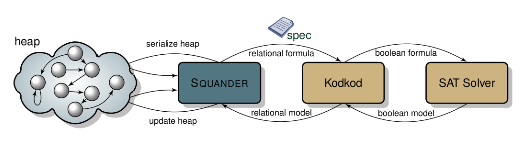
\includegraphics[width=2in]{img/architecture-diagram} 
   \end{center}
 \end{figure}
  %\column{2in}
  
  %\end{columns}
\end{frame}

\subsection{Kodkod}

\begin{frame}
  \frametitle{Kodkod}   % Insert frame title between curly braces
  \begin{itemize}
  \item<1-> solver pro relační logiku
  \item<2-> požaduje ohraničení pro každou relaci a relační formuli
  \item<3-> překládá daný problém do SAT 
  \item<4-> používá SAT solver k nalezení vyhovujícího řešení, které vrací,
  pokud je nalezeno
  \end{itemize}
  %\begin{columns}[c]
  %\column{0.1in}
  %\column{3.1in}
  %\framebox{\includegraphics[height=2.1in]{img/use_case}
 %}
 %\begin{figure}[h]
	%\begin{center}
    %	\includegraphics[height=2.1in]{img/use_case}
    %\end{center}
%\end{figure}
 %\end{columns}
\end{frame}

\subsection{JFSL}

\begin{frame}
  \frametitle{JFSL}   % Insert frame title between curly braces
%  \begin{columns}[c]
%  \column{2in}  % slides are 3in high by 5in wide
  \begin{itemize}
  \item<1-> specifikace pro Javu podporující relační a množinovou algebru
  \item<2-> pomocí této specifikace je možno deklarovat jaká část heapu se změní
  a jak
  \item<3-> poskytuje algebraické operátory společně s celočíselnými operátory a
  booleovskými operátory
  \end{itemize}
%  \column{2in}
  %\framebox{ \includegraphics[height=2.1in]{img/uml}
  %}
%  \begin{figure}[h]
%	\begin{center}
   %\includegraphics[height=2.1in]{img/uml} 
    %\end{center}
  %\end{figure}
  %\end{columns}
\end{frame}

\section{Implementované algoritmy}

\begin{frame}
  \frametitle{Implementované algoritmy}   
  %\begin{columns}[c]
  %\column{2in}  % slides are 3in high by 5in wide
  \begin{block}{Algoritmy naimplementované ve frameworku Squander}
  \begin{itemize}
  \item<1-> Problém batohu
  \item<2-> Zobecněná bisekční šířka
  \item<3-> L-dominující množina grafu
  \item<4-> Nalezení Hamiltonovské cesty
  \item<5-> Trojúhelníkový soliter
  \item<6-> Problém $n$ dam 
  \end{itemize}
  \end{block}
  %\column{2in}
  %\framebox{Insert graphic here % e.g. \includegraphics[height=2.65in]{graphic}
  %}
  %\end{columns}
\end{frame}



\begin{frame}
  \frametitle{Nalezení Hamiltonovské cesty}   
  
  \lstinputlisting[label=hp1,caption=Implementace nalezení Hamiltonovské
cesty ve Squanderu]{src/Hp.java}
  
\end{frame}




\section{Porovnání}

\begin{frame}
  \frametitle{Porovnání}   % Insert frame title between curly braces
  
  \begin{itemize}
  \item<1-> k zvolené sadě algoritmů byly naimplementovány jejich
  \uv{imperativní protějšky}
  \item<2-> imperativní algoritmy byly naimplementovány technikou BB-DFS
  (L-dominující množina grafu,\ldots) nebo pomocí bactrackingu (Nalezení
  Hamiltonovské cesty)
  \item<3-> k jednotlivým algoritmům byly vygenerovány instance daného problému,
  které sloužily k porovnání výpočetního času, zatížení procesoru a paměťové
  náročnosti daného algoritmu v dané implementaci
  \end{itemize}
  
\end{frame}

\begin{frame}
  \frametitle{Porovnání výpočetních časů}
\begin{figure}[h]

	\begin{center}
   	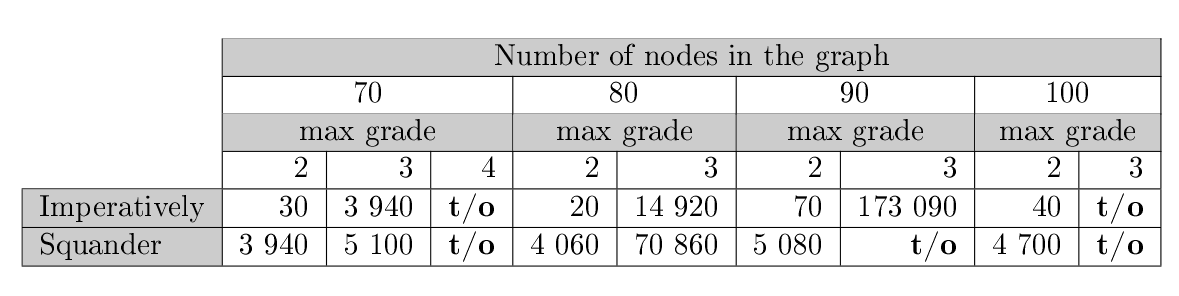
\includegraphics[width=4in]{img/exec-times} 
   \end{center}
   \caption{\tiny Výpočetní časy jednotlivých instancí obou implementací Nalezení
Hamiltonovské cesty}
 \end{figure}  

  
\end{frame}

\begin{frame}
  \frametitle{Paměťová náročnost - imperativní implementace}

\begin{figure}
%\begin{center}
\resizebox{0.7\textwidth}{!}{% GNUPLOT: LaTeX picture with Postscript
\begingroup
  \makeatletter
  \providecommand\color[2][]{%
    \GenericError{(gnuplot) \space\space\space\@spaces}{%
      Package color not loaded in conjunction with
      terminal option `colourtext'%
    }{See the gnuplot documentation for explanation.%
    }{Either use 'blacktext' in gnuplot or load the package
      color.sty in LaTeX.}%
    \renewcommand\color[2][]{}%
  }%
  \providecommand\includegraphics[2][]{%
    \GenericError{(gnuplot) \space\space\space\@spaces}{%
      Package graphicx or graphics not loaded%
    }{See the gnuplot documentation for explanation.%
    }{The gnuplot epslatex terminal needs graphicx.sty or graphics.sty.}%
    \renewcommand\includegraphics[2][]{}%
  }%
  \providecommand\rotatebox[2]{#2}%
  \@ifundefined{ifGPcolor}{%
    \newif\ifGPcolor
    \GPcolorfalse
  }{}%
  \@ifundefined{ifGPblacktext}{%
    \newif\ifGPblacktext
    \GPblacktexttrue
  }{}%
  % define a \g@addto@macro without @ in the name:
  \let\gplgaddtomacro\g@addto@macro
  % define empty templates for all commands taking text:
  \gdef\gplbacktext{}%
  \gdef\gplfronttext{}%
  \makeatother
  \ifGPblacktext
    % no textcolor at all
    \def\colorrgb#1{}%
    \def\colorgray#1{}%
  \else
    % gray or color?
    \ifGPcolor
      \def\colorrgb#1{\color[rgb]{#1}}%
      \def\colorgray#1{\color[gray]{#1}}%
      \expandafter\def\csname LTw\endcsname{\color{white}}%
      \expandafter\def\csname LTb\endcsname{\color{black}}%
      \expandafter\def\csname LTa\endcsname{\color{black}}%
      \expandafter\def\csname LT0\endcsname{\color[rgb]{1,0,0}}%
      \expandafter\def\csname LT1\endcsname{\color[rgb]{0,1,0}}%
      \expandafter\def\csname LT2\endcsname{\color[rgb]{0,0,1}}%
      \expandafter\def\csname LT3\endcsname{\color[rgb]{1,0,1}}%
      \expandafter\def\csname LT4\endcsname{\color[rgb]{0,1,1}}%
      \expandafter\def\csname LT5\endcsname{\color[rgb]{1,1,0}}%
      \expandafter\def\csname LT6\endcsname{\color[rgb]{0,0,0}}%
      \expandafter\def\csname LT7\endcsname{\color[rgb]{1,0.3,0}}%
      \expandafter\def\csname LT8\endcsname{\color[rgb]{0.5,0.5,0.5}}%
    \else
      % gray
      \def\colorrgb#1{\color{black}}%
      \def\colorgray#1{\color[gray]{#1}}%
      \expandafter\def\csname LTw\endcsname{\color{white}}%
      \expandafter\def\csname LTb\endcsname{\color{black}}%
      \expandafter\def\csname LTa\endcsname{\color{black}}%
      \expandafter\def\csname LT0\endcsname{\color{black}}%
      \expandafter\def\csname LT1\endcsname{\color{black}}%
      \expandafter\def\csname LT2\endcsname{\color{black}}%
      \expandafter\def\csname LT3\endcsname{\color{black}}%
      \expandafter\def\csname LT4\endcsname{\color{black}}%
      \expandafter\def\csname LT5\endcsname{\color{black}}%
      \expandafter\def\csname LT6\endcsname{\color{black}}%
      \expandafter\def\csname LT7\endcsname{\color{black}}%
      \expandafter\def\csname LT8\endcsname{\color{black}}%
    \fi
  \fi
  \setlength{\unitlength}{0.0500bp}%
  \begin{picture}(7200.00,5040.00)%
    \gplgaddtomacro\gplbacktext{%
      \csname LTb\endcsname%
      \put(1078,704){\makebox(0,0)[r]{\strut{} 0}}%
      \csname LTb\endcsname%
      \put(1078,1439){\makebox(0,0)[r]{\strut{} 5}}%
      \csname LTb\endcsname%
      \put(1078,2174){\makebox(0,0)[r]{\strut{} 10}}%
      \csname LTb\endcsname%
      \put(1078,2910){\makebox(0,0)[r]{\strut{} 15}}%
      \csname LTb\endcsname%
      \put(1078,3645){\makebox(0,0)[r]{\strut{} 20}}%
      \csname LTb\endcsname%
      \put(1078,4380){\makebox(0,0)[r]{\strut{} 25}}%
      \csname LTb\endcsname%
      \put(1210,484){\makebox(0,0){\strut{} 0}}%
      \csname LTb\endcsname%
      \put(1839,484){\makebox(0,0){\strut{} 10}}%
      \csname LTb\endcsname%
      \put(2468,484){\makebox(0,0){\strut{} 20}}%
      \csname LTb\endcsname%
      \put(3097,484){\makebox(0,0){\strut{} 30}}%
      \csname LTb\endcsname%
      \put(3726,484){\makebox(0,0){\strut{} 40}}%
      \csname LTb\endcsname%
      \put(4354,484){\makebox(0,0){\strut{} 50}}%
      \csname LTb\endcsname%
      \put(4983,484){\makebox(0,0){\strut{} 60}}%
      \csname LTb\endcsname%
      \put(5612,484){\makebox(0,0){\strut{} 70}}%
      \csname LTb\endcsname%
      \put(6241,484){\makebox(0,0){\strut{} 80}}%
      \csname LTb\endcsname%
      \put(6870,484){\makebox(0,0){\strut{} 90}}%
      \put(440,2542){\rotatebox{90}{\makebox(0,0){\strut{}used heap [Mb]}}}%
      \put(4040,154){\makebox(0,0){\strut{}time [s]}}%
      \put(4040,4710){\makebox(0,0){\strut{}Heap memory usage}}%
    }%
    \gplgaddtomacro\gplfronttext{%
    }%
    \gplbacktext
\put(0,0){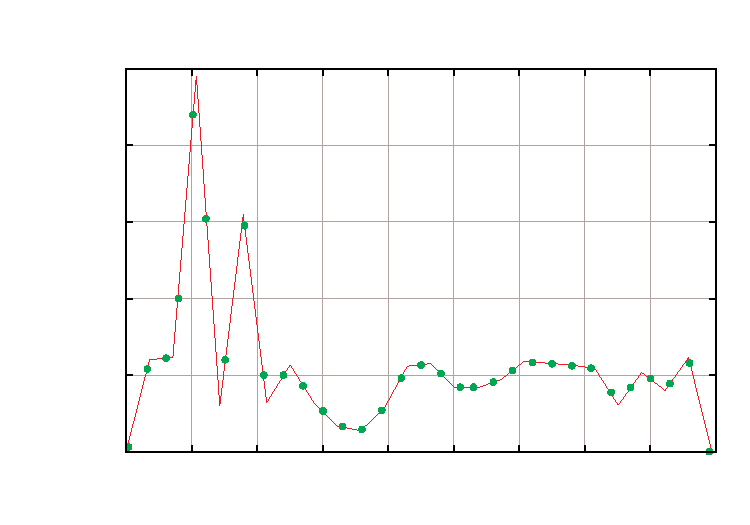
\includegraphics{figures/heap-ldsg-i-50-2-2}}%
    \gplfronttext
  \end{picture}%
\endgroup}

\caption{\tiny Využití heap v čase - Nalezení Hamiltonovské
cesty v imperativní implementataci pro graf se 40 uzly, maximálním stupněm 5}
\label{fig:hpIMem405}
%\end{center}
\end{figure}

\end{frame}


\begin{frame}
  \frametitle{Paměťová náročnost - Squander}

\begin{figure}
%\begin{center}
\resizebox{0.7\textwidth}{!}{% GNUPLOT: LaTeX picture with Postscript
\begingroup
  \makeatletter
  \providecommand\color[2][]{%
    \GenericError{(gnuplot) \space\space\space\@spaces}{%
      Package color not loaded in conjunction with
      terminal option `colourtext'%
    }{See the gnuplot documentation for explanation.%
    }{Either use 'blacktext' in gnuplot or load the package
      color.sty in LaTeX.}%
    \renewcommand\color[2][]{}%
  }%
  \providecommand\includegraphics[2][]{%
    \GenericError{(gnuplot) \space\space\space\@spaces}{%
      Package graphicx or graphics not loaded%
    }{See the gnuplot documentation for explanation.%
    }{The gnuplot epslatex terminal needs graphicx.sty or graphics.sty.}%
    \renewcommand\includegraphics[2][]{}%
  }%
  \providecommand\rotatebox[2]{#2}%
  \@ifundefined{ifGPcolor}{%
    \newif\ifGPcolor
    \GPcolorfalse
  }{}%
  \@ifundefined{ifGPblacktext}{%
    \newif\ifGPblacktext
    \GPblacktexttrue
  }{}%
  % define a \g@addto@macro without @ in the name:
  \let\gplgaddtomacro\g@addto@macro
  % define empty templates for all commands taking text:
  \gdef\gplbacktext{}%
  \gdef\gplfronttext{}%
  \makeatother
  \ifGPblacktext
    % no textcolor at all
    \def\colorrgb#1{}%
    \def\colorgray#1{}%
  \else
    % gray or color?
    \ifGPcolor
      \def\colorrgb#1{\color[rgb]{#1}}%
      \def\colorgray#1{\color[gray]{#1}}%
      \expandafter\def\csname LTw\endcsname{\color{white}}%
      \expandafter\def\csname LTb\endcsname{\color{black}}%
      \expandafter\def\csname LTa\endcsname{\color{black}}%
      \expandafter\def\csname LT0\endcsname{\color[rgb]{1,0,0}}%
      \expandafter\def\csname LT1\endcsname{\color[rgb]{0,1,0}}%
      \expandafter\def\csname LT2\endcsname{\color[rgb]{0,0,1}}%
      \expandafter\def\csname LT3\endcsname{\color[rgb]{1,0,1}}%
      \expandafter\def\csname LT4\endcsname{\color[rgb]{0,1,1}}%
      \expandafter\def\csname LT5\endcsname{\color[rgb]{1,1,0}}%
      \expandafter\def\csname LT6\endcsname{\color[rgb]{0,0,0}}%
      \expandafter\def\csname LT7\endcsname{\color[rgb]{1,0.3,0}}%
      \expandafter\def\csname LT8\endcsname{\color[rgb]{0.5,0.5,0.5}}%
    \else
      % gray
      \def\colorrgb#1{\color{black}}%
      \def\colorgray#1{\color[gray]{#1}}%
      \expandafter\def\csname LTw\endcsname{\color{white}}%
      \expandafter\def\csname LTb\endcsname{\color{black}}%
      \expandafter\def\csname LTa\endcsname{\color{black}}%
      \expandafter\def\csname LT0\endcsname{\color{black}}%
      \expandafter\def\csname LT1\endcsname{\color{black}}%
      \expandafter\def\csname LT2\endcsname{\color{black}}%
      \expandafter\def\csname LT3\endcsname{\color{black}}%
      \expandafter\def\csname LT4\endcsname{\color{black}}%
      \expandafter\def\csname LT5\endcsname{\color{black}}%
      \expandafter\def\csname LT6\endcsname{\color{black}}%
      \expandafter\def\csname LT7\endcsname{\color{black}}%
      \expandafter\def\csname LT8\endcsname{\color{black}}%
    \fi
  \fi
  \setlength{\unitlength}{0.0500bp}%
  \begin{picture}(7200.00,5040.00)%
    \gplgaddtomacro\gplbacktext{%
      \csname LTb\endcsname%
      \put(1078,704){\makebox(0,0)[r]{\strut{} 0}}%
      \csname LTb\endcsname%
      \put(1078,1439){\makebox(0,0)[r]{\strut{} 5}}%
      \csname LTb\endcsname%
      \put(1078,2174){\makebox(0,0)[r]{\strut{} 10}}%
      \csname LTb\endcsname%
      \put(1078,2910){\makebox(0,0)[r]{\strut{} 15}}%
      \csname LTb\endcsname%
      \put(1078,3645){\makebox(0,0)[r]{\strut{} 20}}%
      \csname LTb\endcsname%
      \put(1078,4380){\makebox(0,0)[r]{\strut{} 25}}%
      \csname LTb\endcsname%
      \put(1210,484){\makebox(0,0){\strut{} 0}}%
      \csname LTb\endcsname%
      \put(1839,484){\makebox(0,0){\strut{} 10}}%
      \csname LTb\endcsname%
      \put(2468,484){\makebox(0,0){\strut{} 20}}%
      \csname LTb\endcsname%
      \put(3097,484){\makebox(0,0){\strut{} 30}}%
      \csname LTb\endcsname%
      \put(3726,484){\makebox(0,0){\strut{} 40}}%
      \csname LTb\endcsname%
      \put(4354,484){\makebox(0,0){\strut{} 50}}%
      \csname LTb\endcsname%
      \put(4983,484){\makebox(0,0){\strut{} 60}}%
      \csname LTb\endcsname%
      \put(5612,484){\makebox(0,0){\strut{} 70}}%
      \csname LTb\endcsname%
      \put(6241,484){\makebox(0,0){\strut{} 80}}%
      \csname LTb\endcsname%
      \put(6870,484){\makebox(0,0){\strut{} 90}}%
      \put(440,2542){\rotatebox{90}{\makebox(0,0){\strut{}used heap [Mb]}}}%
      \put(4040,154){\makebox(0,0){\strut{}time [s]}}%
      \put(4040,4710){\makebox(0,0){\strut{}Heap memory usage}}%
    }%
    \gplgaddtomacro\gplfronttext{%
    }%
    \gplbacktext
\put(0,0){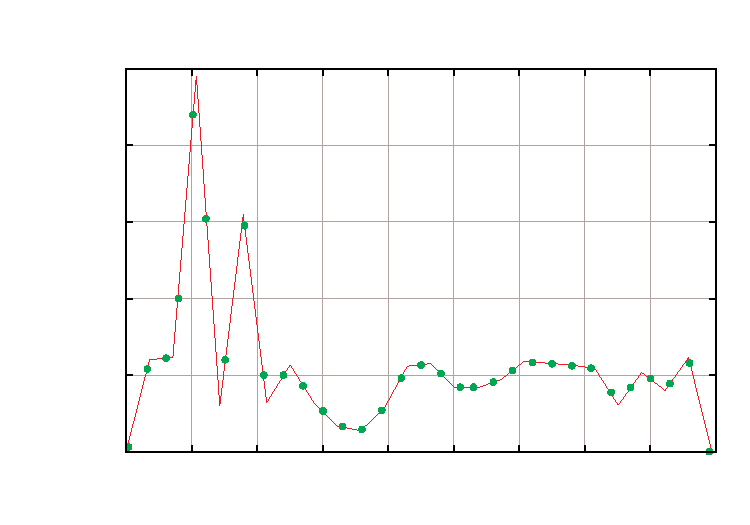
\includegraphics{figures/heap-ldsg-i-50-2-2}}%
    \gplfronttext
  \end{picture}%
\endgroup}

\caption{\tiny Využití heap v čase - Nalezení Hamiltonovské
cesty v implementataci frameworkem Squander pro graf se 40 uzly, maximálním
stupněm 5}
\label{fig:hpIMem405}
%\end{center}
\end{figure}

\end{frame}



\begin{frame}
  \frametitle{Zatížení procesoru - imperativní implementace}
\begin{figure}
%\begin{center}
\resizebox{0.7\textwidth}{!}{% GNUPLOT: LaTeX picture with Postscript
\begingroup
  \makeatletter
  \providecommand\color[2][]{%
    \GenericError{(gnuplot) \space\space\space\@spaces}{%
      Package color not loaded in conjunction with
      terminal option `colourtext'%
    }{See the gnuplot documentation for explanation.%
    }{Either use 'blacktext' in gnuplot or load the package
      color.sty in LaTeX.}%
    \renewcommand\color[2][]{}%
  }%
  \providecommand\includegraphics[2][]{%
    \GenericError{(gnuplot) \space\space\space\@spaces}{%
      Package graphicx or graphics not loaded%
    }{See the gnuplot documentation for explanation.%
    }{The gnuplot epslatex terminal needs graphicx.sty or graphics.sty.}%
    \renewcommand\includegraphics[2][]{}%
  }%
  \providecommand\rotatebox[2]{#2}%
  \@ifundefined{ifGPcolor}{%
    \newif\ifGPcolor
    \GPcolorfalse
  }{}%
  \@ifundefined{ifGPblacktext}{%
    \newif\ifGPblacktext
    \GPblacktexttrue
  }{}%
  % define a \g@addto@macro without @ in the name:
  \let\gplgaddtomacro\g@addto@macro
  % define empty templates for all commands taking text:
  \gdef\gplbacktext{}%
  \gdef\gplfronttext{}%
  \makeatother
  \ifGPblacktext
    % no textcolor at all
    \def\colorrgb#1{}%
    \def\colorgray#1{}%
  \else
    % gray or color?
    \ifGPcolor
      \def\colorrgb#1{\color[rgb]{#1}}%
      \def\colorgray#1{\color[gray]{#1}}%
      \expandafter\def\csname LTw\endcsname{\color{white}}%
      \expandafter\def\csname LTb\endcsname{\color{black}}%
      \expandafter\def\csname LTa\endcsname{\color{black}}%
      \expandafter\def\csname LT0\endcsname{\color[rgb]{1,0,0}}%
      \expandafter\def\csname LT1\endcsname{\color[rgb]{0,1,0}}%
      \expandafter\def\csname LT2\endcsname{\color[rgb]{0,0,1}}%
      \expandafter\def\csname LT3\endcsname{\color[rgb]{1,0,1}}%
      \expandafter\def\csname LT4\endcsname{\color[rgb]{0,1,1}}%
      \expandafter\def\csname LT5\endcsname{\color[rgb]{1,1,0}}%
      \expandafter\def\csname LT6\endcsname{\color[rgb]{0,0,0}}%
      \expandafter\def\csname LT7\endcsname{\color[rgb]{1,0.3,0}}%
      \expandafter\def\csname LT8\endcsname{\color[rgb]{0.5,0.5,0.5}}%
    \else
      % gray
      \def\colorrgb#1{\color{black}}%
      \def\colorgray#1{\color[gray]{#1}}%
      \expandafter\def\csname LTw\endcsname{\color{white}}%
      \expandafter\def\csname LTb\endcsname{\color{black}}%
      \expandafter\def\csname LTa\endcsname{\color{black}}%
      \expandafter\def\csname LT0\endcsname{\color{black}}%
      \expandafter\def\csname LT1\endcsname{\color{black}}%
      \expandafter\def\csname LT2\endcsname{\color{black}}%
      \expandafter\def\csname LT3\endcsname{\color{black}}%
      \expandafter\def\csname LT4\endcsname{\color{black}}%
      \expandafter\def\csname LT5\endcsname{\color{black}}%
      \expandafter\def\csname LT6\endcsname{\color{black}}%
      \expandafter\def\csname LT7\endcsname{\color{black}}%
      \expandafter\def\csname LT8\endcsname{\color{black}}%
    \fi
  \fi
  \setlength{\unitlength}{0.0500bp}%
  \begin{picture}(7200.00,5040.00)%
    \gplgaddtomacro\gplbacktext{%
      \csname LTb\endcsname%
      \put(1078,704){\makebox(0,0)[r]{\strut{} 0}}%
      \csname LTb\endcsname%
      \put(1078,1229){\makebox(0,0)[r]{\strut{} 10}}%
      \csname LTb\endcsname%
      \put(1078,1754){\makebox(0,0)[r]{\strut{} 20}}%
      \csname LTb\endcsname%
      \put(1078,2279){\makebox(0,0)[r]{\strut{} 30}}%
      \csname LTb\endcsname%
      \put(1078,2805){\makebox(0,0)[r]{\strut{} 40}}%
      \csname LTb\endcsname%
      \put(1078,3330){\makebox(0,0)[r]{\strut{} 50}}%
      \csname LTb\endcsname%
      \put(1078,3855){\makebox(0,0)[r]{\strut{} 60}}%
      \csname LTb\endcsname%
      \put(1078,4380){\makebox(0,0)[r]{\strut{} 70}}%
      \csname LTb\endcsname%
      \put(1210,484){\makebox(0,0){\strut{} 0}}%
      \csname LTb\endcsname%
      \put(2019,484){\makebox(0,0){\strut{} 100}}%
      \csname LTb\endcsname%
      \put(2827,484){\makebox(0,0){\strut{} 200}}%
      \csname LTb\endcsname%
      \put(3636,484){\makebox(0,0){\strut{} 300}}%
      \csname LTb\endcsname%
      \put(4444,484){\makebox(0,0){\strut{} 400}}%
      \csname LTb\endcsname%
      \put(5253,484){\makebox(0,0){\strut{} 500}}%
      \csname LTb\endcsname%
      \put(6061,484){\makebox(0,0){\strut{} 600}}%
      \csname LTb\endcsname%
      \put(6870,484){\makebox(0,0){\strut{} 700}}%
      \put(440,2542){\rotatebox{90}{\makebox(0,0){\strut{}CPU used [\%]}}}%
      \put(4040,154){\makebox(0,0){\strut{}time [s]}}%
      \put(4040,4710){\makebox(0,0){\strut{}CPU usage}}%
    }%
    \gplgaddtomacro\gplfronttext{%
    }%
    \gplbacktext
    \put(0,0){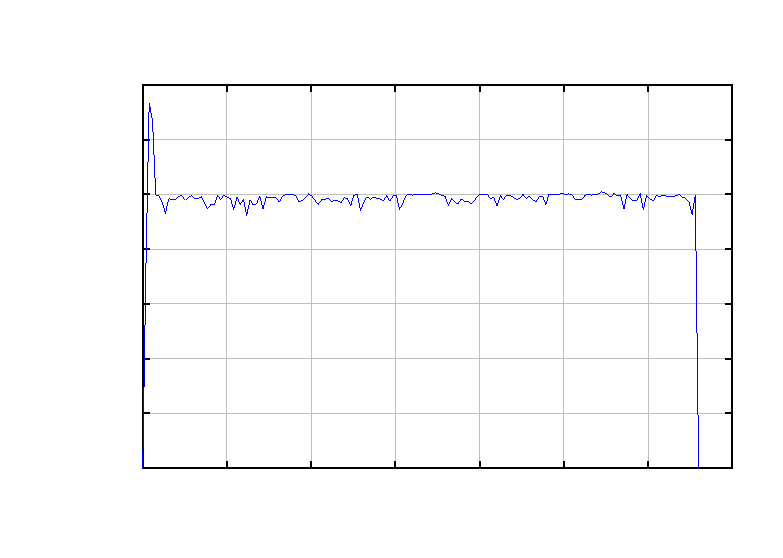
\includegraphics{figures/cpu-hp-s-40-5}}%
    \gplfronttext
  \end{picture}%
\endgroup}

\caption{\tiny Zatížení procesoru v čase - Nalezení Hamiltonovské
cesty v imperativní implementataci pro graf se 40 uzly, maximálním stupněm 5}
\label{fig:hpIMem405}
%\end{center}
\end{figure}
\end{frame}


\begin{frame}
  \frametitle{Zatížení procesoru - Squander}
\begin{figure}
%\begin{center}
\resizebox{0.7\textwidth}{!}{% GNUPLOT: LaTeX picture with Postscript
\begingroup
  \makeatletter
  \providecommand\color[2][]{%
    \GenericError{(gnuplot) \space\space\space\@spaces}{%
      Package color not loaded in conjunction with
      terminal option `colourtext'%
    }{See the gnuplot documentation for explanation.%
    }{Either use 'blacktext' in gnuplot or load the package
      color.sty in LaTeX.}%
    \renewcommand\color[2][]{}%
  }%
  \providecommand\includegraphics[2][]{%
    \GenericError{(gnuplot) \space\space\space\@spaces}{%
      Package graphicx or graphics not loaded%
    }{See the gnuplot documentation for explanation.%
    }{The gnuplot epslatex terminal needs graphicx.sty or graphics.sty.}%
    \renewcommand\includegraphics[2][]{}%
  }%
  \providecommand\rotatebox[2]{#2}%
  \@ifundefined{ifGPcolor}{%
    \newif\ifGPcolor
    \GPcolorfalse
  }{}%
  \@ifundefined{ifGPblacktext}{%
    \newif\ifGPblacktext
    \GPblacktexttrue
  }{}%
  % define a \g@addto@macro without @ in the name:
  \let\gplgaddtomacro\g@addto@macro
  % define empty templates for all commands taking text:
  \gdef\gplbacktext{}%
  \gdef\gplfronttext{}%
  \makeatother
  \ifGPblacktext
    % no textcolor at all
    \def\colorrgb#1{}%
    \def\colorgray#1{}%
  \else
    % gray or color?
    \ifGPcolor
      \def\colorrgb#1{\color[rgb]{#1}}%
      \def\colorgray#1{\color[gray]{#1}}%
      \expandafter\def\csname LTw\endcsname{\color{white}}%
      \expandafter\def\csname LTb\endcsname{\color{black}}%
      \expandafter\def\csname LTa\endcsname{\color{black}}%
      \expandafter\def\csname LT0\endcsname{\color[rgb]{1,0,0}}%
      \expandafter\def\csname LT1\endcsname{\color[rgb]{0,1,0}}%
      \expandafter\def\csname LT2\endcsname{\color[rgb]{0,0,1}}%
      \expandafter\def\csname LT3\endcsname{\color[rgb]{1,0,1}}%
      \expandafter\def\csname LT4\endcsname{\color[rgb]{0,1,1}}%
      \expandafter\def\csname LT5\endcsname{\color[rgb]{1,1,0}}%
      \expandafter\def\csname LT6\endcsname{\color[rgb]{0,0,0}}%
      \expandafter\def\csname LT7\endcsname{\color[rgb]{1,0.3,0}}%
      \expandafter\def\csname LT8\endcsname{\color[rgb]{0.5,0.5,0.5}}%
    \else
      % gray
      \def\colorrgb#1{\color{black}}%
      \def\colorgray#1{\color[gray]{#1}}%
      \expandafter\def\csname LTw\endcsname{\color{white}}%
      \expandafter\def\csname LTb\endcsname{\color{black}}%
      \expandafter\def\csname LTa\endcsname{\color{black}}%
      \expandafter\def\csname LT0\endcsname{\color{black}}%
      \expandafter\def\csname LT1\endcsname{\color{black}}%
      \expandafter\def\csname LT2\endcsname{\color{black}}%
      \expandafter\def\csname LT3\endcsname{\color{black}}%
      \expandafter\def\csname LT4\endcsname{\color{black}}%
      \expandafter\def\csname LT5\endcsname{\color{black}}%
      \expandafter\def\csname LT6\endcsname{\color{black}}%
      \expandafter\def\csname LT7\endcsname{\color{black}}%
      \expandafter\def\csname LT8\endcsname{\color{black}}%
    \fi
  \fi
  \setlength{\unitlength}{0.0500bp}%
  \begin{picture}(7200.00,5040.00)%
    \gplgaddtomacro\gplbacktext{%
      \csname LTb\endcsname%
      \put(1078,704){\makebox(0,0)[r]{\strut{} 0}}%
      \csname LTb\endcsname%
      \put(1078,1229){\makebox(0,0)[r]{\strut{} 10}}%
      \csname LTb\endcsname%
      \put(1078,1754){\makebox(0,0)[r]{\strut{} 20}}%
      \csname LTb\endcsname%
      \put(1078,2279){\makebox(0,0)[r]{\strut{} 30}}%
      \csname LTb\endcsname%
      \put(1078,2805){\makebox(0,0)[r]{\strut{} 40}}%
      \csname LTb\endcsname%
      \put(1078,3330){\makebox(0,0)[r]{\strut{} 50}}%
      \csname LTb\endcsname%
      \put(1078,3855){\makebox(0,0)[r]{\strut{} 60}}%
      \csname LTb\endcsname%
      \put(1078,4380){\makebox(0,0)[r]{\strut{} 70}}%
      \csname LTb\endcsname%
      \put(1210,484){\makebox(0,0){\strut{} 0}}%
      \csname LTb\endcsname%
      \put(2019,484){\makebox(0,0){\strut{} 100}}%
      \csname LTb\endcsname%
      \put(2827,484){\makebox(0,0){\strut{} 200}}%
      \csname LTb\endcsname%
      \put(3636,484){\makebox(0,0){\strut{} 300}}%
      \csname LTb\endcsname%
      \put(4444,484){\makebox(0,0){\strut{} 400}}%
      \csname LTb\endcsname%
      \put(5253,484){\makebox(0,0){\strut{} 500}}%
      \csname LTb\endcsname%
      \put(6061,484){\makebox(0,0){\strut{} 600}}%
      \csname LTb\endcsname%
      \put(6870,484){\makebox(0,0){\strut{} 700}}%
      \put(440,2542){\rotatebox{90}{\makebox(0,0){\strut{}CPU used [\%]}}}%
      \put(4040,154){\makebox(0,0){\strut{}time [s]}}%
      \put(4040,4710){\makebox(0,0){\strut{}CPU usage}}%
    }%
    \gplgaddtomacro\gplfronttext{%
    }%
    \gplbacktext
    \put(0,0){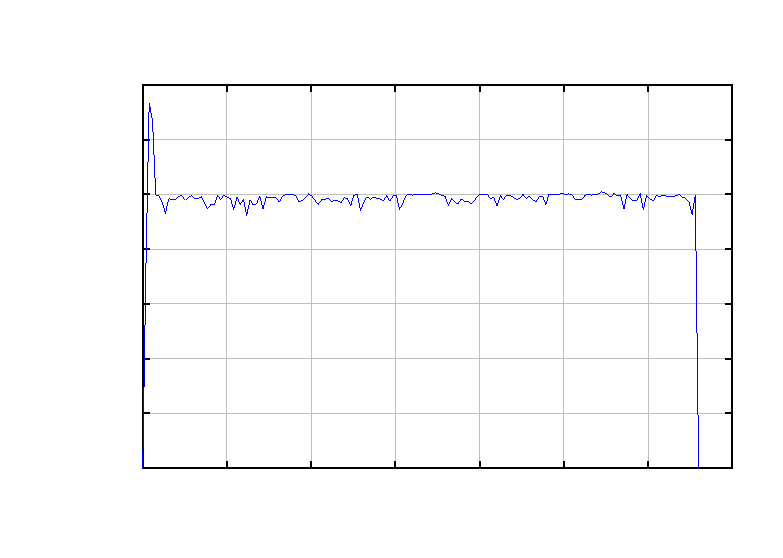
\includegraphics{figures/cpu-hp-s-40-5}}%
    \gplfronttext
  \end{picture}%
\endgroup}

\caption{\tiny Zatížení procesoru v čase - Nalezení Hamiltonovské
cesty v implementataci frameworkem Squander pro graf se 40 uzly, maximálním stupněm 5}
\label{fig:hpIMem405}
%\end{center}
\end{figure}
\end{frame}

\begin{frame}
\frametitle{Činnost garbage collectoru}
\begin{figure}[h]
	\begin{center}
	
   	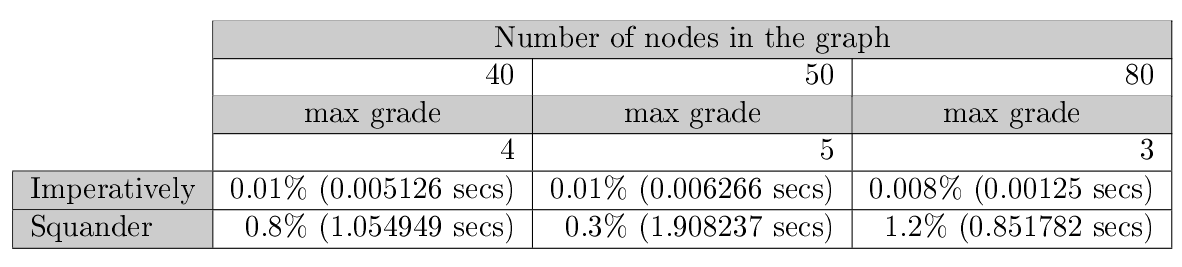
\includegraphics[width=4in]{img/gc-activity} 
   \end{center}
   \caption{\tiny Poměr časové činnosti garbage collectoru ku celkovému
	výpočetnímu času u implementací Nalezení Hamiltonovské cesty}
 \end{figure}
\end{frame}

\begin{frame}
\frametitle{Porovnání závislostí}
\begin{itemize}
  \item<1-> pro implementaci ve Squanderu podle vypočítaných korelací závisí
  výpočetní čas více na maximálním stupni uzlu v grafu - hodnota korelace 0.91 -
  než na počtu uzlů v grafu - hodnota korelace 0.48
  \item<2-> pro imperativní implementaci podle vypočítaných
  korelací závisí trochu více výpočetní čas na počtu uzlů v grafu - hodnota
  korelace 0.48 - než na maximálním stupni uzlu v grafu - hodnota korelace 0.44
  \end{itemize}
\end{frame}

\section{Zhodnocení}

\begin{frame}
  \frametitle{Zhodnocení (1)}
  \begin{itemize}
  \item<1-> Squander je zajímavý nástroj pro programování problémů obsahujících
  mnoho závislostí
  \item<2-> JFSL poskytuje dostatečné množství výrazů pro implementaci algoritmů
  \item<3-> díky frameworku lze současně snadno využít výhod jak imperativního,
  tak deklarativního programování
  \item<4-> při programování občas nastává problém se scopem celočíselných
  proměnných
  \end{itemize}
\end{frame}



\begin{frame}
  \frametitle{Zhodnocení (2)}
  \begin{itemize}  
  
  \item<1-> framework podporuje pouze first order logic
  \item<2-> při použití frameworku dochází samozřejmě k větší paměťové zátěži
  než při imperativním programování, nicméně zátěž na procesor je podobná
  \item<3-> výpočetní čas implementace ve frameworku je závislý na jiných
  parametrech instance než je tomu u imperativní implementace
  \item<4-> programování ve frameworku lze v praxi využít např. pro programování
  rozvrhů, kontroly studijního plánu a jiných problémů obsahujících velké
  množství závislostí
  \end{itemize}
  \end{frame}





\note{The end}       % Add notes to yourself that will be displayed when
		     % typeset with the notes or notesonly class options

\end{document}